% !TEX root = ../main.tex
% chktex-file 21
% chktex-file 46
\section{Spectral Graph Theory}%
\label{sec:sgt}

We start with an introduction to spectral graph theory, which will allow us to characterize and compare the structure of graphs.
Graphs are most commonly described in their vertex base, i.e.\  the connection strength $w_{i j}$ of pairs $(v_i, v_j)$ of vertices.
\begin{align}
	G :=&\, (\mathcal{V}, \mathcal{E}, W)\quad\text{with } W \in \mathbb{R}^{N \times N}, N := |\mathcal{V}|
\end{align}
In this paper we will only consider undirected graphs with non-negative real weights and without self-loops ($\forall v_i: w_{i i} = 0$).

The core idea of spectral graph theory is to perform a change of basis of $W$ and describe graphs in terms of their so called \textit{spectral base} instead of their \textit{vertex base}.
To see what this means, we interpret the adjacency/weight matrix $W$ as a linear operator that operates on so called signals $x \in \mathbb{R}^N$.
A signal $x$ can be interpreted as a function $x: \mathcal{V} \to \mathbb{R}$ that assigns a signal strength to each vertex.
By applying $Wx$ the given signal strengths $x_i$ are shifted according to the connection strenghts $w_{i j}$ to neighboring vertices $v_j$.
This interpretation of graphs is very similar to that of Markov chains where signals represent probability distributions.

\subsection{Relating Graph Signals to Real-valued Functions}%
\label{sec:sgt:real}

Let us now compare discrete graph signals $x: \mathcal{V} \to \mathbb{R}$ to continuous real-valued functions $f: \mathbb{R} \to \mathbb{R}$.
Both only differ in their domain.
The domain $\mathbb{R}$ of $f$ has an inherent structure, the real number line, which provides a strict ordering of its elements and a notion of distance between them.
The domain $\mathcal{V}$ of $x$ however has no such inherent structure, i.e.\  $v_1 < v_2$ for two vertices $v_1, v_2$ does not have a clear meaning.
The structure of $\mathcal{V}$ fully depends on the graph $G$ that is acting on it.
Intuitively graph signals can thus be understood as a discretized generalization of real-valued functions, where the underlying structure of the input domain is not fixed but can be freely chosen.
\begin{figure}[ht]
	\centering
	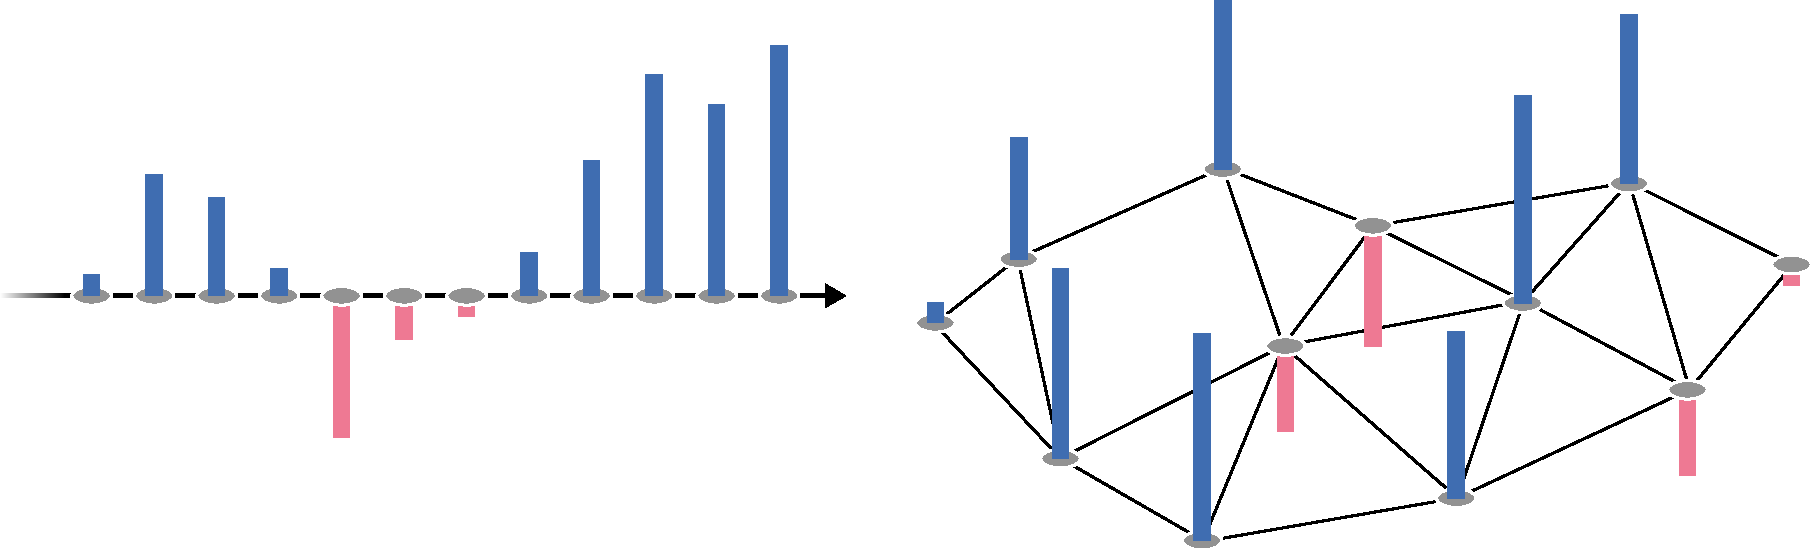
\includegraphics[width=0.8\linewidth]{gfx/sgt/real-graph.pdf}
	\caption{%
		Illustration of how the discretized real number line can be interpreted as an infinite linear graph, compared to some arbitrary finite non-linear graph.
		The bars show the signal strengths $f(t)$ and $x_i$ at the vertices $b_t$ and $b_i$ respectively.
	}\label{fig:sgt:realGraph}
\end{figure}

\Cref{fig:sgt:realGraph} shows that all real-valued functions $f$ can be seen as signals $x$ of the graph described by the real number line\footnote{%
	Technically this is not correct, since $\mathbb{R}$ is continuous whereas all vertex sets $\mathcal{V}$ have to be discrete.
	To build an intuition for graph signals, this detail can however be ignored.
}.
Both, real-valued functions and graph signals, can be described as vectors in their time and vertex base respectively:
\begin{equation}
	\begin{split}
		f = \int_{\mathbb{R}} f(t) b_t dt
		\Rightarrow \langle b_t, f \rangle = f(t)
	\end{split}
	\quad\text{and}\quad
	\begin{split}
		x = \sum_{i = 1}^{N} x_i b_i
		\Rightarrow \langle b_i, x \rangle = x_i
	\end{split}
\end{equation}
In this equation ${\{ b_i \}}_{v_i \in \mathcal{V}}$ denotes the standard basis of the adjacency matrix $W$, i.e.\ $b_i \in \mathbb{R}^N$ has a signal strength of $0$ for all $v_{j \neq i}$ and a signal strength of $1$ for $v_i$.
Similarly ${\{ b_t \}}_{t \in \mathbb{R}}$ denotes the infinite dimensional standard basis of the space of real functions, where $\langle b_t, \cdot \rangle := \delta_t(\cdot)$, with $\delta$ denoting the Dirac delta function.

\subsection{Extending the Fourier Transform to Graphs}%
\label{sec:sgt:fourier}

As mentioned at the beginning of this section, the core idea of spectral graph theory is to express graph signal vectors $x$ in the spectral basis ${\{ u_i \}}_{i = 1}^{N}$ instead of the standard vertex basis ${\{ b_i \}}_{v_i \in \mathcal{V}}$.
This idea is analogous to the classical Fourier transform on real-valued functions.
In the first step we are now going to give an intuition for the classical Fourier transform.
Afterwards we will extend this intuition to the graph domain.

The Fourier basis ${\{ u_\xi \}}_{\xi \in \mathbb{R}}$ describes a function $f$ not in terms of the values $f(t) = \langle b_t, f \rangle$ it takes at position $t$ but instead in terms of the amplitudes $\hat{f}(\xi) = \langle u_\xi, f \rangle$ of the complex exponentials $u_\xi(t) = e^{2\pi i \xi t}$.
Using this perspective, the Fourier transform can be viewed as a change of basis operator from the orthonormal standard basis ${\{ b_t \}}_{t \in \mathbb{R}}$ to the also orthonormal Fourier basis ${\{ u_\xi \}}_{\xi \in \mathbb{R}}$:
\begin{align}
	f = \int_{\mathbb{R}} \underbrace{\langle b_t, f \rangle}_{f(t)} b_t dt\quad=\quad\int_{\mathbb{R}} \underbrace{\langle u_\xi, f \rangle}_{\hat{f}(\xi)} u_\xi d\xi
\end{align}
This property of the Fourier transform by itself is not special; in fact there are infinitely many orthonormal bases on the space of real-valued functions.
The distinguishing property of ${\{ u_\xi \}}_{\xi \in \mathbb{R}}$, making it useful in many domains, is that it is an \textit{eigenbasis} of the \textit{Laplacian} $\Updelta$, i.e.\  $\Updelta u_\xi = \lambda_\xi u_\xi$ for the eigenvalue $\lambda_\xi \in \mathbb{R}$.
The Laplacian is a multi\-dimensional generalization of the second derivative.
For real-valued functions this boils down to $\Updelta u_\xi = \frac{\partial^2}{\partial t^2} u_\xi = -{(2 \pi \xi)}^2 e^{2 \pi i \xi t}$ with the eigenvalue $\lambda_\xi = {-(2\pi\xi)}^2$ depending solely on the frequency $\xi$.
The original motivation to express functions in terms of the Laplacian's eigenbasis was to solve the physical heat equation\footnote{%
	More generally the Fourier basis turns out to be meaningful for all \textit{linear time-invariant} (LTI) systems, of which the heat equations are only one instance.
}.
For this reason it is a useful intuition to think about signals as temperature distributions that will converge to an equilibrium state over time.
This intuition also works in the graph setting where heat only flows between neighboring vertices in proportion to their connection strengths.

Now that we have looked at the Fourier transform of real-valued functions, we will extend this notion to graphs.
Just like the classical Fourier transform, the graph Fourier transform performs a change of basis of a signal $x$ from the vertex basis ${\{ b_i \}}_{v_i \in \mathcal{V}}$ to the Fourier basis ${\{ u_k \}}_{k = 1}^{N}$.
This Fourier basis again is characterized by it being an eigenbasis of the Laplacian, more specifically the so called \textit{combinatorial graph Laplacian} $L$ in this case:
\begin{align}
	L := D - W\quad\text{with the degree matrix } D := {
		\renewcommand*{\arraystretch}{0.5}
		\begin{pmatrix}
			d_1 & & \\
			& \ddots & \\
			& & d_N
		\end{pmatrix}
	}, d_i := \sum_{j = 1}^{N} w_{i j}
\end{align}
Using this definition, the application $L x$ is a discrete generalized analogue of the second derivative $\frac{\partial^2}{\partial t^2} f$.
Putting both Laplacian variants, $\frac{\partial^2}{\partial t^2}$ and $L$, side-by-side gives an intuition for why this is the case:
\begin{equation}
	\begin{split}
		\left(-\frac{\partial^2}{\partial t^2} f\right)\mkern-4mu(t) = \lim_{h \to 0} \frac{1}{h^2} (\underbrace{f(t) - f(t-h)}_{\Delta_{t, t-h}} + \underbrace{f(t) -  f(t+h)}_{\Delta_{t, t+h}})
	\end{split}
	\begin{split}\ \left|\ %
		{(L x)}_i = \sum_{j = 1}^{N} w_{i j} \underbrace{(x_i - x_j)}_{\Delta_{i, j}}
	\right.\end{split}
\end{equation}
The second derivative of a function $f$ essentially just averages the differences in signal strength in the neighborhood of a point $f(t)$.
For real-valued functions this neighborhood only consists of the two infinitesimally close points to the left and to the right of a point, i.e.\ $f(t - h)$ and $f(t + h)$.
The graph Laplacian represents the same operation, where each point/vertex might however have more than two neighbors that need to be averaged.

Based on the graph Laplacian $L$ we just defined, the graph Fourier basis ${\{ u_k \}}_{k = 1}^{N}$ is just the set of eigenvectors of $L$.
In the rest of this paper we will assume that these eigenvectors $u_k$ are sorted in ascending order w.r.t.\  their eigenvalues $\lambda_k$, i.e.\  $\lambda_1 \leq \lambda_2 \leq \cdots \leq \lambda_N$.
\Cref{fig:sgt:graphFourier} shows how this definition generalizes the Fourier basis from the real number line to an arbitrary graph.
It also shows that the eigenvalues $\lambda_k$ of the graph Fourier basis encode some notion of frequency, just like they do for the classical Fourier basis.
Analogous to the classical Fourier transform, the eigenvalues of a graph's Laplacian are therefore also called its \textit{spectrum}.
\begin{figure}[ht]
	\centering
	\makebox[\textwidth][c]{\includegraphics[width=\linewidth]{gfx/sgt/graph-fourier.pdf}}
	\caption{%
		Comparison between the basis functions/vectors of the classical Fourier transform and the graph Fourier transform.
		For the eigenfunctions on the upper half only the real cosine components of the complex exponentials are shown.
		\source[based on]{Shuman2013}
	}\label{fig:sgt:graphFourier}
\end{figure}

\subsection{Spectral Properties of Graphs}%
\label{sec:sgt:spectrum}

We will now give an intuition for the relation between the spectrum of a graph and its structural properties\footnote{%
	Only a general overview will be given. For a more detailed discussion we refer to \citet{Shuman2013}.
}.
For any graph the smallest eigenvalue always is $\lambda_1 = 0$ with the associated eigenvector $u_1 = \frac{1}{\sqrt{N}} {(1, \dots, 1)}^\top$ being a uniform signal over all vertices.
Using the heat analogy, this simply means that any system in which everything has the same temperature is in an equilibrium state and no heat is flowing.
More generally for graphs with $m$ separate connected components the first $m$ eigenvalues are all $0$ since each component can have its own equilibrium temperature without causing heat flow.
If the spectrum of a graph is known, this fact can be used to quickly determine whether a graph is connected or not.

Another meaningful eigenvalue is $\lambda_2$ and its eigenvector $u_2$, also called the \textit{Fiedler value} and \textit{Fiedler vector} respectively.
As we have just seen, a Fiedler value of $\lambda_2 = 0$ means that a graph is not connected.
More generally the Fielder value can be interpreted as a measure of overall graph connectivity\footnote{%
	Formally this measure is called \textit{algebraic connectivity}, as opposed to regular \textit{graph connectivity}, which is defined as $\min_{v_i \in \mathcal{V}} \deg(v_i)$.
}.
If there are two clusters of vertices $\mathcal{V}_+$ and $\mathcal{V}_-$ in a graph that are connected via relatively few edges (compared to the overall number of edges), the Fielder value is small;
for well connected graphs on the other hand the Fiedler value is large.
Using the heat analogy, the Fielder value essentially measures the ``width'' of a bottleneck between two parts of a graph through which heat will only flow very slowly or even not at all in case of $\lambda_2 = 0$.
The partitioning of vertices into $\mathcal{V}_+$ and $\mathcal{V}_-$ can be retrieved via the Fiedler vector $u_2$;
vertices with a positive signal strength in $u_2$ are in $\mathcal{V}_+$, the other vertices are in $\mathcal{V}_-$.
The so called \textit{spectral clustering} algorithm is based on this relationship.
\Cref{fig:sgt:graphFourier} shows how the Fiedler vector $u_2$ partitions a graph via the signs of the vertex signal strengths.

As we have just seen, expressing a graph $G$ in terms of the spectrum of its Laplacian $L$ gives access to graph characteristics like its overall connectivity.
Similarly to how the low-frequency components of the Fourier transform of a function represent the overall shape of that function, the eigenvectors associated with the small eigenvalues of $L$ represent overall characteristics of $G$.
The details of a function or graph on the other hand are encoded in the high-frequency components of its Fourier transform, i.e.\  the eigenvectors associated with large eigenvalues.
This perspective already hints at how spectral graph analysis might be useful to approximate graphs.
